
\documentclass[DIV=calc, paper=a4, fontsize=11pt, twocolumn, spanish]{scrartcl}	 % A4 paper and 11pt font size

\usepackage{lipsum} % Used for inserting dummy 'Lorem ipsum' text into the template
\usepackage[protrusion=true,expansion=true]{microtype} % Better typography
\usepackage{amsmath,amsfonts,amsthm} % Math packages
\usepackage[svgnames]{xcolor} % Enabling colors by their 'svgnames'
\usepackage[hang, small,labelfont=bf,up,textfont=it,up]{caption} % Custom captions under/above floats in tables or figures
\usepackage{booktabs} % Horizontal rules in tables
\usepackage{fix-cm}	 % Custom font sizes - used for the initial letter in the document
\usepackage[spanish]{babel}
\selectlanguage{spanish}
\usepackage[utf8]{inputenc}
\usepackage{graphicx}

\usepackage{sectsty} % Enables custom section titles
\allsectionsfont{\usefont{OT1}{phv}{b}{n}} % Change the font of all section commands

\usepackage{fancyhdr} % Needed to define custom headers/footers
\pagestyle{fancy} % Enables the custom headers/footers
\usepackage{lastpage} % Used to determine the number of pages in the document (for "Page X of Total")

% Headers - all currently empty
\lhead{}
\chead{}
\rhead{}

% Footers
\lfoot{}
\cfoot{}
\rfoot{\footnotesize Page \thepage\ of \pageref{LastPage}} % "Page 1 of 2"

\renewcommand{\headrulewidth}{0.0pt} % No header rule
\renewcommand{\footrulewidth}{0.4pt} % Thin footer rule

\usepackage{lettrine} % Package to accentuate the first letter of the text
\newcommand{\initial}[1]{ % Defines the command and style for the first letter
\lettrine[lines=3,lhang=0.3,nindent=0em]{
\color{DarkGoldenrod}
{\textsf{#1}}}{}}

%----------------------------------------------------------------------------------------
%	TITLE SECTION
%----------------------------------------------------------------------------------------

\usepackage{titling} % Allows custom title configuration

\newcommand{\HorRule}{\color{DarkGoldenrod} \rule{\linewidth}{1pt}} % Defines the gold horizontal rule around the title

\pretitle{\vspace{-30pt} \begin{flushleft} \HorRule \fontsize{35}{35} \usefont{OT1}{phv}{b}{n} \color{DarkRed} \selectfont} % Horizontal rule before the title

\title{Gas ideal} % Your article title

\posttitle{\par\end{flushleft}\vskip 0.2em} % Whitespace under the title

\preauthor{\begin{flushleft}\large \lineskip 0.5em \usefont{OT1}{phv}{b}{sl} \color{DarkRed}} % Author font configuration

\author{Sebastián Valencia, } % Your name

\postauthor{\footnotesize \usefont{OT1}{phv}{m}{sl} \color{Black} % Configuration for the institution name
Universidad de los Andes \\ 201111578

\par\end{flushleft}\HorRule} % Horizontal rule after the title



\date{} % Add a date here if you would like one to appear underneath the title block

%----------------------------------------------------------------------------------------

\begin{document}

\maketitle % Print the title

\thispagestyle{fancy} % Enabling the custom headers/footers for the first page 

%----------------------------------------------------------------------------------------
%	ABSTRACT
%----------------------------------------------------------------------------------------

% The first character should be within \initial{}
\initial{U}\textbf{n gas ideal es un gas teórico compuesto de un conjunto de partículas puntuales con desplazamiento aleatorio que no interactuan entre sí. El concepto de gas ideal es útil porque el mismo se comporta según la ley de los gases ideales, una ecuación de estado simplificada, y que puede ser analizada mediante la mecánica estadística.} Tomado de: \cite{Wikipedia}

%----------------------------------------------------------------------------------------
%	ARTICLE CONTENTS
%----------------------------------------------------------------------------------------

\section*{Objetivos}

\begin{enumerate}
\item Estudiar la relación entre la presión, el volumen y la temperatura de una muestra de aire.
\item Estimar el cero absoluto de temperatura.
\end{enumerate}


\section*{Teoría}

\begin{figure}[htbp]
\centering
	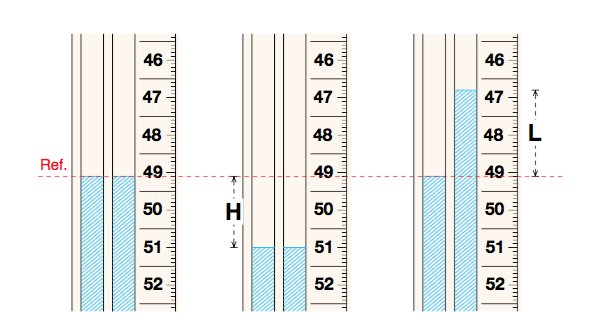
\includegraphics[scale=0.7]{data/img/proc}
	\caption{En el estudio de la muestra de aire a presión constante deben igualarse los dos niveles bajando el extremo libre de la manguera. En el estudio a volumen constante se debe subir hasta que el nivel 1 regrese a la altura de referencia.}
\end{figure}

Presión hidrostatica: $\Delta P = \rho g \Delta h$. Comportamiento de gases ideales. Cero absoluto de temperatura.\\

\begin{enumerate}
\item En términos de $H$ encontrar la ecuación que representa al volumen total de la muestra de aire. ¿Qué otras dos cantidades además de $H$ son necesarias?

\vspace{40 mm}

\item En términos de $L$ y la presión atmosférica en el laboratorio $P_0$, encontrar la ecuación para hallar la presión absoluta del gas en el escenario donde el volumen se mantiene constante.

\vspace{40 mm}

\item 
Consultar el valor de la presión atmosférica en Bogotá.
\end{enumerate}

\section*{Procedimiento experimental}

\begin{figure}[htbp]
\centering
	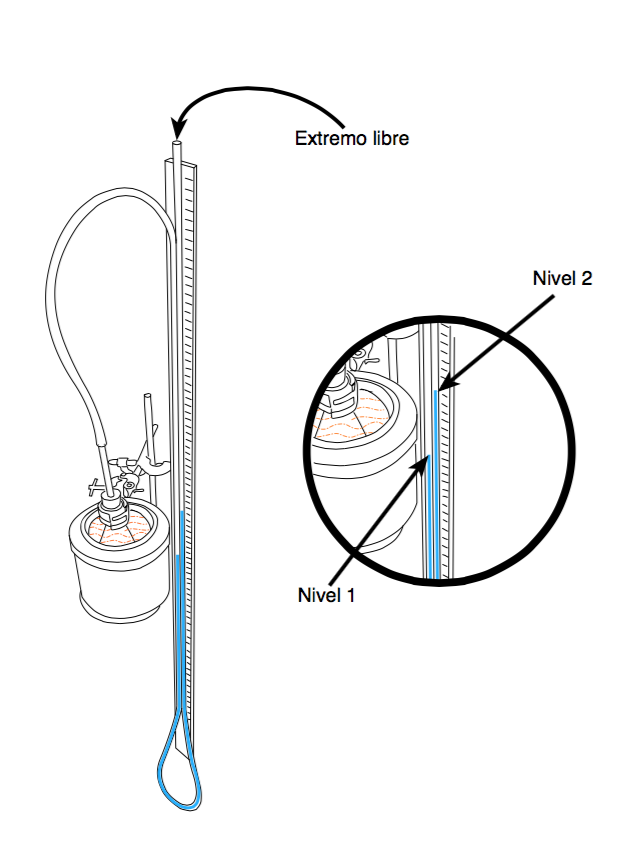
\includegraphics[scale=0.5]{data/img/disp}
	\caption{Disposición de elementos para el desarrollo del laboratorio. Señalización de los niveles.}
\end{figure}

En este experimento tomamos una muestra de aire con temperatura controlada para determinar el comportamiento de su presión cuando su volumen permanece constante, y el del volumen cuando la presión se mantiene fija. La muestra de aire a estudiar esta contenida en un matraz y en un segmento de manguera; el agua sirve el doble propósito de aprisionar la muestra de aire y de servir como testigo de la presión manometrica de la misma. Llamamos \textit{nivel 1} al nivel que esta en contacto con la muestra de aire, y \textit{nivel 2} al que esta en contacto con el aire del laboratorio.\\

En el experimento regulamos la temperatura de la muestra de aire modificando la temperatura de un reservorio ter mico que rodea al matraz que lo contiene. Para controlar la presión se mueve el extremo libre de la manguera hasta que los dos niveles de agua se igualan, el nivel 1 indica el aumento de volumen del gas. Para controlar el volumen se mueve el extremo libre hasta que el nivel 1 regresa a su posición inicial; la diferencia de los dos niveles señala la presión manometrica del aire.\\

Con los datos a presión y volumen constantes, hacemos en cada uno una extrapolación para estimar el cero absoluto de temperatura, que en el escenario de presión constante corresponde a la temperatura a la cual el volumen se anula, y que en el caso de volumen constante corresponde a la temperatura a la cual la presión se anula. Los materiales necesarios son:

\begin{itemize}
\item Calorímetro
\item Matraz Erlenmeyer con tapón y manguera
\item Termómetro
\item Regla
\item Agua
\item Jeringa
\item Termómetro
\item Horno
\item Soporte universal
\end{itemize}

La cantidad de agua en la manguera debe ser tal que ocupe entre 50 y 100 cm. Inicialmente el matraz debe estar inmerso en agua fría. Si se tiene disponible un barómetro en el laboratorio usar su lectura para la presión atmosférica, de lo contrario utilice el valor consultado.\\

Con la manguera desconectada del matraz movemos el extremo libre de la manguera hacia arriba o hacia abajo hasta dejar el nivel inicial cerca del centro de la regla o un poco más abajo. Conectamos con firmeza la manguera al matraz y no la desconectamos durante todo el experimento. Ponemos una gota de agua en el borde del matraz que sirva como indicador de alguna fuga. Al conectar la manguera los dos niveles cambian un poco, volvemos a igualarlos manipulando el extremo libre, una vez igualados registramos la altura correspondiente en la regla; esta será la altura de referencia para todo el experimento.\\

%----------------------------------------------------------------------------------------
%	REFERENCE LIST
%----------------------------------------------------------------------------------------

\begin{thebibliography}{99} % Bibliography - this is intentionally simple in this template

  \bibitem{young2011sears} Sears and Zemansky.B. {\em Sears and Zemansky's University Physics / Tutorials in Introductory Physics / Tutorials in Introductory Physics Homework. 17:565--567}, Pearson Education.  2011.
  
  \bibitem{Wikipedia} \textit{https://es.wikipedia.org/wiki/Gas\_ideal}, Consultado en Febrero 2016.
 
\end{thebibliography}

%----------------------------------------------------------------------------------------

\end{document}